\documentclass[
	a4paper,
	oneside,
	% BCOR = 10mm,
	DIV = 14,
	fontsize = 14pt,
	headings = normal,
]{scrartcl}

%%% Length calculations
\usepackage{calc}
%%%

%%% Support for color
\usepackage{xcolor}
\definecolor{lightblue}{HTML}{03A9F4}
\definecolor{red}{HTML}{F44336}
%%%

%%% Including graphics
\usepackage{graphicx}
%%%

%%% Font selection
\usepackage{fontspec}

\setromanfont{STIX Two Text}[
	SmallCapsFeatures = {LetterSpace = 8},
]

\setsansfont{IBM Plex Sans}[
	Scale = MatchUppercase,
]

\setmonofont{IBM Plex Mono}[
	Scale = MatchUppercase,
]
%%%

%%% Math typesetting
\usepackage{amsmath}

\usepackage{unicode-math}
\setmathfont{STIX Two Math}

\usepackage{IEEEtrantools}
%%%

%%% List settings
\usepackage{enumitem}
\setlist[enumerate]{
	label*      = {\arabic*.},
	leftmargin  = *,
	labelindent = \parindent,
	topsep      = 1\baselineskip,
	parsep      = 0\baselineskip,
	itemsep     = 1\baselineskip,
	noitemsep,
}

\setlist[itemize]{
	label*      = {—},
	leftmargin  = *,
	labelindent = \parindent,
	topsep      = 1\baselineskip,
	parsep      = 0\baselineskip,
	itemsep     = 1\baselineskip,
	noitemsep,
}

\setlist[description]{
	font        = {\rmfamily\upshape\bfseries},
	topsep      = 1\baselineskip,
	parsep      = 0\baselineskip,
	itemsep     = 0\baselineskip,
	noitemsep,
}

%%%

%%% Structural elements typesetting
\setkomafont{pagenumber}{\rmfamily}
\setkomafont{disposition}{\rmfamily\bfseries}

% Sectioning
\RedeclareSectionCommand[
	beforeskip = -1\baselineskip,
	afterskip  = 1\baselineskip,
	font       = {\normalsize\bfseries\scshape},
]{section}

\RedeclareSectionCommand[
	beforeskip = -1\baselineskip,
	afterskip  = 1\baselineskip,
	font       = {\normalsize\bfseries\itshape},
]{subsection}

\RedeclareSectionCommand[
	beforeskip = -1\baselineskip,
	afterskip  = 1\baselineskip,
	font       = {\normalsize\bfseries},
]{subsubsection}

\RedeclareSectionCommand[
	beforeskip = -1\baselineskip,
	afterskip  = -0.5em,
	font       = {\normalsize\mdseries\scshape\addfontfeatures{Letters = {UppercaseSmallCaps}}},
]{paragraph}
%%%

%%% Typographic enhancements
\usepackage{microtype}
%%%

%%% Language-specific settings
\usepackage{polyglossia}
\setmainlanguage{ukrainian}
\setotherlanguages{english,russian}
%%%

%%% Captions
\usepackage{caption}
\usepackage{subcaption}

%\DeclareCaptionLabelFormat{closing}{#2)}
%\captionsetup[subtable]{labelformat = closing}

%\captionsetup[subfigure]{labelformat = closing}

\captionsetup[table]{
	aboveskip = 0\baselineskip,
	belowskip = 0\baselineskip,
}

\captionsetup[figure]{
	aboveskip = 1\baselineskip,
	belowskip = 0\baselineskip,
}

\captionsetup[subfigure]{
	labelformat = simple,
	labelformat = brace,
}
%%%

%%% Hyphenated ragged typesetting
\usepackage{ragged2e}
%%%

%%% Table typesetting
\usepackage{booktabs}
\usepackage{longtable}

\usepackage{multirow}

\usepackage{array}
\newcolumntype{v}[1]{>{\RaggedRight\arraybackslash\hspace{0pt}}p{#1}}
\newcolumntype{b}[1]{>{\Centering\arraybackslash\hspace{0pt}}p{#1}}
\newcolumntype{n}[1]{>{\RaggedLeft\arraybackslash\hspace{0pt}}p{#1}}
%%%

%%% Drawing
\usepackage{tikz}
\usepackage{tikzscale}
\usetikzlibrary{positioning}
\usetikzlibrary{arrows.meta} % Stealth arrow tips
%%%

%%% SI units typesetting
\usepackage{siunitx}
\sisetup{
	output-decimal-marker = {,},
	exponent-product      = {\cdot},
	inter-unit-product    = \ensuremath{{} \cdot {}},
	per-mode              = symbol,
}

\DeclareSIUnit\flops{\text{FLOPS}}
\DeclareSIUnit\bit{\text{бит}}
\DeclareSIUnit\byte{\text{байт}}

%%%

%%% Links and hyperreferences
\usepackage{hyperref}
\hypersetup{
	bookmarksnumbered = true,
	colorlinks      = false,
	linkbordercolor = red,
	urlbordercolor  = lightblue,
	pdfborderstyle  = {/S/U/W 1.5},
}
%%%

%%% Length adjustments
% Set baselineskip, default is 14.5 pt
\linespread{1.068966} % ~15.5 pt
\setlength{\emergencystretch}{1em}
\setlength{\parindent}{1.5em}
\newlength{\gridunitwidth}
\setlength{\gridunitwidth}{\textwidth / 12}
%%%

%%% Boldface math in sectioning commands
\makeatletter
\g@addto@macro\bfseries{\boldmath}
\makeatother
%%%

%%% Custom commands
\newcommand{\allcaps}[1]{{\addfontfeatures{LetterSpace = 8, Kerning = Off}#1}}
\newcommand{\filename}[1]{\texttt{\textenglish{#1}}}
\newcommand{\regkey}[1]{\texttt{\textenglish{#1}}}
%%%

\begin{document}
\setlength{\RaggedRightParindent}{\parindent}
\RaggedRight

	\section{Понятие сложной динамической системы}

	\section{Основные признаки сложной системы или ТУ}
		\subsection{Конспект}
		\begin{russian}
			Можно обозначить основные признаки сложного технического устройства. Выделяют несколько:
		\begin{enumerate}
			\item Обладание определённым единством целей и~выработка оптимальных выходных сигналов при~наличии множества входных сигналов.
			\item Выполнение большого количества различных функций, которые осуществляются множеством частей, входящих в~это техническое устройство.
			\item Сложность функционирования: изменение одной переменной на~входе ведёт за~собой изменение многих переменных на~выходе.
			\item Высокая степень автоматизации. 
			\item Возможность описания поступающего на~вход технического устройства возмущения только статистически. Имеется в~виду, что для того, чтобы описать работу технического устройства, недостаточно одного эксперимента~— необходимо несколько.
		\end{enumerate}
		\end{russian}

	\section{Понятие эксплуатации сложного ТУ}
		\subsection{Конспект}
		\begin{russian}
			Эксплуатация сложного технического устройства~— это процесс использования его по~назначению и~поддержание его в~технически исправном состоянии. Содержание в~исправном состоянии заключается в~ряде мероприятий, требующего непрерывного воздействия на~техническое устройство, для~поддержания его в~рабочем состоянии. К~таким мероприятиям относятся:
			\begin{itemize}
				\item плановое техническое обслуживание;
				\item восстановление после сбоя;
				\item подготовка к работе после хранения.
			\end{itemize}
		\end{russian}

		\subsection{Литература}
			Експлуатація~— це організовані дії технічного персоналу з~доведення засобу чи систем до~необхідного стану працездатності чи збереження, підтримання їх у~цьому стані і~використання з~необхідним рівнем ефективності.

			Процес експлуатації полягає у~виконанні робіт з~транспортування, збереження підготовки до~використання, використання, контролю, ремонту та~технічного обслуговування.

	\section{Надежность как свойство сложного ТУ}
	\begin{russian}
		\subsection{Конспект}
			Под \emph{надёжностью} понимают свойство технического устройства~(ТУ) выполнять заданные функции, сохраняя свои эксплуатационные показатели в~заданных пределах в~течение требуемого промежутка времени и~требуемой наработки в~определённых условиях эксплуатации. \emph{Наработка}~— требуемый промежуток времени, когда работает устройство. Эта надёжность понимается в~определённых условиях эксплуатации.
	\end{russian}

		\subsection{Литература}
			Надійність~— це властивість засобу зберігати тривалий час в~установлених межах значення всіх параметрів, які характеризують здатність використовувати необхідні функції в~заданих режимах і~умовах використання, технічного обслуговування, ремонту, зберігання і~транспортування. Ця властивість залежно від призначення засобу й умов його використанні об'єднує в~собі властивості безвідмовності, довгостроковості, ремонтоздатності і~збереженості.

	\section{Понятие работоспособности ТУ}
		\subsection{Конспект}
		\begin{russian}
			\emph{Работоспособность} — это состояние технического устройства, при котором оно способно выполнять заданные функции с параметрами, установленными технической документацией. 
		\end{russian}

		\subsection{Литература}
			Справність~— це стан засобу чи системи, за якого він відповідає всім вимогам нормативно-технічної документації.

	\section{Проблемы обеспечения надежности ТУ}
		\subsection{Конспект}
		\begin{russian}
			Проблема надёжности технического устройства имеет два аспекта:
			\begin{enumerate}
				\item Количественное определение надёжности.
				\item Обеспечение требуемого уровня надёжности в~процессе эксплуатации.
			\end{enumerate}

		\end{russian}

	\section{Понятие «отказ ТУ»}
		\subsection{Конспект}
		\begin{russian}
			В качестве отправных данных при определении количественных значений надёжности используются события, которые заключаются в~нарушении работоспособности технического устройства. Такие события называются отказами. Под \emph{отказом} понимают событие, после которого техническое устройство перестаёт выполнять свои функции полностью или частично. 
		\end{russian}

		\subsection{Литература}
			Відмова~— це подія, котра призводить до~порушення працездатності засобу чи системи.

	\section{Понятие долговечности}
		\subsection{Конспект}
		\begin{russian}
			Долговечность~— свойство технического устройства сохранять работоспособность с необходимыми перерывами для технического обслуживания и ремонта вплоть до~предельного состояния, оговоренного в~технической документации.
		\end{russian}

		\subsection{Литература}
			Довговічність~— це властивість обладнання зберігати працездатність до~настання граничного стану з~можливими перервами в~роботі, пов'язаними з~ремонтом і~технічним обслуговуванням.

	\section{Восстанавливаемые и невосстанавливаемые ТУ}
		Відновлювані технічні засоби~— це такі технічні засоби, що у~випадку виникнення відмови можуть бути відновлені. 

		Невідновлювані технічні засоби~— це такі технічні засоби, що у~випадку виникнення відмови або не підлягають, або не піддається відновленню.

	\section{Сроком службы ТУ}
		\subsection{Литература}
			Строк служби~— це календарна тривалість експлуатації засобу від її початку до~настання граничного стану незалежно від його напрацювання.

	\section{Вероятность безотказной работы ТУ}
		\subsection{Литература}
			Імовірність безвідмовної роботи $P(t)$~— це ймовірність того, що протягом заданого напрацювання відмова засобу не відбудеться за умови його працездатності в~початковий момент. Математично вона найчастіше оцінюється так:
			\[
				P(t) = \exp{\left( -\int_{0}^{t} \omega(u)\,du \right)}.
			\]
			При $\omega(t) = \lambda$ отримуємо $P(t) = \exp(-\lambda t)$. Якщо $t = 0$, то~$P(t) = 1$; при $t = T_0$ одержуємо $P(t) = 0.37$; при $t = \infty$~маємо $P(t) = 0$.

		\subsection{Конспект}

	\section{Интенсивность отказов}
		\subsection{Литература}
			Інтерсивність відмов обчислюється як кількість відмов апаратури за одиницю часу в~період її нормальної експлуатації, коли інтенсивність відмов має постійне значення. При цьому статистично вона визначається як:
			\[
				\lambda = \frac{1}{T_{\text{СНВ}}}.
			\]
			де $T_{\text{СНВ}}$~— середнє напрацювання на~відмову.

	\section{«Среднее время безотказной работы»}
		Середнє напрацювання на~відмову (середній час безвідмовної роботи)~— це математичне сподівання випадкового напрацювання апаратури між послідовними відмовами. Зазвичай~$T_{\text{СНВ}}$ використовується в~період сталого процесу експлуатації і~статистично визначається як:
			\[
				T_{\text{СНВ}} = \frac{1}{n} \sum_{i = 1}^{n} t_i,
			\]
			де $t_i$~— відрізок часу безвідмовної роботи між двома послідовними відмовами, $1 < i < n$; $n$~— кількість відмов протягом роботи системи. При цьому:
			\[
				t_{\text{р}} = \sum_{i = 1}^{n} t_i,
			\]
			де $t_{\text{р}}$~— загальний час роботи системи.

	\section{Плотность распределения времени безотказной работы}
		Плотность распределения времени безотказной работы~— безусловная плотность вероятности отказов за бесконечно малый интервал времени:
		\[
			f(t) = P(t) \lambda(t).
		\]

	\section{Функции надежности и ненадежности}

	\section{Характеристики надежности невосстанавливаемых ТУ и связь между ними}
		Основними нормованими показниками надійності невідновлюваних ТЗ можуть бути такі показники:
	\begin{enumerate}
		\item Ймовірність безвідмовної роботи~$P(t)$;
		\item Ймовірність відмови~$Q(t)$;
		\item Частота відмов~$a(t)$;
		\item Інтенсивність відмов~$\lambda (t)$;
		\item Середнє напрацювання до~першої відмови~$T_{\text{ср}}$.
	\end{enumerate}

		Оскільки час настання відмови $T$ є величина випадкова, то~$Q(t)$~— це ймовірність того, що випадкова величина $Т$ набуде значення, менше або рівне $t$~(інтегральна функція розподілу відмов), де~$t$~— час, за який визначається показник надійності, тобто ймовірністю відмови називається ймовірність того, що за певних умов експлуатації в~заданому інтервалі часу виникне хоча б одна відмова:
		\[
			Q(t) = P(T \leqslant t).
		\]

		Ймовірністю безвідмовної роботи~$P(t)$ називається ймовірність того, що за певних умов експлуатації за певних умов експлуатації в~заданому інтервалі часу або у~межах заданого напрацювання~$t$ не відбудеться жодної відмови:
		\[
			P(t) = P(T > t).
		\]

		Оскількe безвідмовна робота і~відмова є подіями неспільними і~протилежними, то~між ними справедливе таке співвідношення:
		\[
			P(t) + Q(t) = 1.
			\]

			Оскільки~$Q(t)$ є законом розподілу випадкової величини (відмов), то~залежність між можливими значеннями безперервної випадкової величини~$T$ та~ймовірностями влучення в~їх межі називається щільністью ймовірності.

			Вважаючи, що в~момент ввімкнення технічний засіб роботоздатний, тобто~$P(0) = 1$, функція~$P(t)$ монотонно спадає від 1 до~0~(рис.~\ref{fig:qt-pt-relation}). При цьому зрозуміло, що~$P(\infty) = 0$, тобто будь-який технічний засіб при~$t \to \infty$ з~часом відмовить.

			\begin{figure}[!htbp]
				\centering
				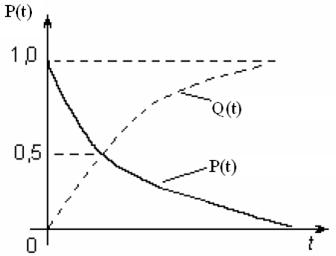
\includegraphics[height = 8\baselineskip]{./assets/qt-pt-relation.jpg}
				\caption{Характеристики зміни ймовірності безвідмовної роботи та~ймовірності відмови}
				\label{fig:qt-pt-relation}
			\end{figure}

			Частота відмов~$a(t)$ є щільністю ймовірності часу роботи технічного засобу до~першої відмови:
			\[
				a(t) = \frac{dQ(t)}{dt} = \frac{-dP(t)}{dt}.
			\]

			Інтенсивністю відмов називається відношення числа відмовлених технічних засобів за одиницю часу до~середнього числа технічних засобів, що справно працюють в~даному проміжку часу. Ймовірнісна оцінка цієї характеристики знаходиться за виразом:
			\begin{equation}
			\label{eq:lambda}
				\lambda = \frac{a(t)}{P(t)}.
			\end{equation}
			Середнім напрацюванням до~першої відмови~$T_{\text{ср}}$ називається математичне сподівання~$M[t]$ часу роботи технічного засобу до~відмови. Математичне сподівання, тобто~$T_{\text{ср}}$, обчислюється за частотою відмов (щільність розподілу часу безвідмовної роботи) так:
			\[
				M[t] = T_{\text{ср}} = \int\limits_{-\infty}^{+\infty} ta(t)\,dt,
			\]
			оскільки $t > 0$ і~$P(0) = 1$, а $P(\infty) = 0$, то~$T_{cр} = \int_{0}^{+\infty} P(t)\,dt$.

			Величина~$T_{\text{ср}}$~— параметр функції~$P(t)$, який в~багатьої випадках дозволяє відновити всю функцію. Інколи середній час безвідмовної роботи~$T_{\text{ср}}$ є прийнятною характеристикою для порівняння технічного засобу за показниками безвідмовності.

			Знаючи один з~показників надійності і~закон розподілу відмов, можна обчислити інші характеристики надійності, враховуючи такі формули:
			\begin{IEEEeqnarray*}{rCl}
				Q(t) &=& \int\limits_{0}^{t} a(t)\,dt,\\
				P(t) &=& 1 - \int\limits_{0}^{t}a(t)\,dt,\\
				P(t) &=& \exp\left( - \int\limits_{0}^{t} \lambda(t)\,dt \right),
			\end{IEEEeqnarray*}
			де~$\lambda(t)$~— інтенсивність відмов, що розраховується за формулою~\eqref{eq:lambda}.

	\section{Кривые распределения времени безотказной работы ТУ}

	\section{Выражение среднего времени безотказной работы ТУ}

	\section{Физическая природа отказов}

	\section{Зависимость интенсивности отказов на~протяжении жизненного цикла ТУ}

	\section{Природа проявления приработочных отказов}

	\section{Характеристика периода износа ТУ}

	\section{Вероятность безотказной работы невосстанавливаемых ТУ}

	\section{Определение среднего времени безотказной работы}

	\section{Виды компьютеров}
		\subsection{Конспект}
			Комп'ютери поділяються на~такі види:
			\begin{enumerate}
				\item Суперкомп'ютер — потужний багатопроцесорний комп'ютер, який має дуже велику продуктивність. Для того, щоб визначити їх продуктивність, існує одиниця \textenglish{FLOPS}. $\SI{1}{\peta\flops} = \SI{10e13}{\flops}$. Наприклад, \textenglish{IBM Roadrunner}~— суперкомп'ютер, розташований в~Інституті фізико-хімічних досліджень у~Кобе, Японія. Його продуктивність~— \SI{11.28}{\peta\flops}. Він складається з~\si{88 128}~8-ядерних процесорів, об'єм оперативної пам'яті~— \SI{80}{\tera\byte}, енергоспоживання~— \SI{12.6}{\mega\watt}, маса~— \SI{226}{\tonne}, площа, яку він займає~— \SI{1100}{\metre\squared}, ціна~— 133~млн~\$.

				\item Мейнфрейм — один головний комп'ютер в~певному обчислювальному центрі.

				\item Кластери комп'ютерів — групи комп'ютерів, фізично розташовані поряд. Їх інколи вважають окремим комп'ютером.

				\item Багатоцільові комп'ютери (комп'ютери загального призначення).

				\item Настільні комп'ютери (\textenglish{desktop}).

				\item Портативні комп'ютери.

				\item Мобільне устаткування (\textenglish{mobile intelligent devices}).

				\item Індивідуальні носимі комп'ютери~— комп'ютер, вбудований в~скафандр космонавта.

				\item Системи реального часу.
			\end{enumerate}

			Обчислювальна машина~— 1 ОС. Реальний час~— це така робота комп'ютера, коли темп обробки інформації в~комп'ютері підпорядковується темпу зміни інформації в~навколишньому середовищі. Наприклад, автоматизовані системи управління повітряним рухом. 

	\section{Понятие технической диагностики}
		\subsection{Конспект}
			Технічна діагностика~— це область знань, що включає відомості про методи і~засоби оцінки технічного стану пристрою. Діагностування технічних об'єктів включає такі функції:
			\begin{enumerate}
				\item Оцінка технічного стану.
				\item Визначення місця локалізації несправності.
				\item Прогнозування залишкового ресурсу.
				\item Моніторинг технічного стану.
			\end{enumerate}

	\section{Диагностические параметры ТУ}
		% Под диагностическими параметрами понимают репрезентативные параметры, по которым можно судить о состоянии объекта. Различают прямые и косвенные диагностические параметры. Первые непосредственно характеризуют состояние объекта, а вторые связаны с прямыми параметрами функциональной зависимостью.

		% При функциональной диагностике объекта в~процессе его работы~— наряду с отдельно рассматриваемыми параметрами~— могут использоваться также как признак состояния функциональные связи (функциональные зависимости) параметров. 

	\section{Проблемы технической диагностики}
			Проблемою технічної діагностики є досягнення адекватної оцінки істинного стану об'єкту і~адекватної оцінки істинного стану і~класифікації цього стану. Для підтвердження нормального стану об'єкту виділяють 2 основні задачі:
			\begin{enumerate}
				\item Забезпечення отримання достовірної інформації.
				\item Забезпечення оперативності її отримання.
			\end{enumerate}

			При виявленні аномалій в~роботі технічного пристрою є 2 проблеми: імовірність пропуску несправності та~імовірність несправедливої тривоги. Чим менше імовірність несправедливої тривоги, тим менша імовірність пропуску і~навпаки.

			Завдання технічної діагностики несправності полягає в~знаходженні «золотої середини» між цими двома проблемами. 

	\section{Средства диагностирования ПК}

	\section{Виды диагностических программ}
		\subsection{Література}
			Для ПК існує кілька видів діагностичних програм (деякі з~них поставляються разом із комп'ютером), що дають змогу користувачу виявляти причини неполадок, що виникають у~комп'ютері. У багатьох випадках такі програми можуть виконати основну роботу з~визначення дефектного взула. Умовно їх можна поділити на~кілька груп, причому складність програм і~їх можливості в~кожній наступній групі вище, ніж у~попередній:
			\begin{enumerate}
				\item \textenglish{POST} (\textenglish{Power-On Self Test})~— процедура самоперевірки при увімкненні, виконується при кожному ввімкненні комп'\-юте\-ра.
				\item Діагностичні програми фірм-ви\-роб\-ни\-ків. Більшість відомих фірм-ви\-роб\-ни\-ків ком\-п'\-юте\-рів випускають для своїх систем спеціалізоване діагностичне програмне забезпечення, що звичайно містить набір тестів, які дають змогу ретельно перевірити усі компоненти ком\-п'\-юте\-ра.
				\item Діагностичні програми фірм-виробників устаткування. Багато виробників устаткування випускають діагностичні програми, призначені для перевірки певного пристрою. Наприклад, фірма \textenglish{Adaptec} випускає програми для перевірки працездатності~\textenglish{SCSI}-адаптерів.
				\item Діагностичні програми операційних систем. Операційні системи \textenglish{Windows}, починаючи з~найперших модифікацій, поставляються з~кількома діагностичними програмами для перевірки різних компонентів ком\-п'\-юте\-ра.
				\item Діагностичні програми загального призначення забезпечують ретельне тестування будь-яких \textenglish{PC}-сумісних ком\-п'юте\-рів.
			\end{enumerate}

	\section{Самопроверка ПК при включении}

	\section{Представление ошибок системой POST}

	\section{Диагностические программы общего назначения}

	\section{Время выполнения задания}

	\section{Диагностические программы операционной системы}

	\section{Диагностика сетевых адаптеров}

	\section{Диагностика компьютера при включении}

	\section{Этап загрузки, не зависящий от типа ОС}
		Процес стандартного завантаження комп'ютера можна розділити на~декілька етапів:
		\begin{enumerate}
			\item Включення живлення.
			\item Джерело живлення виконує самотестування: якщо всі вихідні параметри відповідають нормі, подається сигнал \textenglish{Power Good}. На таку первинну діагностику живлення виділяється \num{0.1}–\SI{0.5}{\second}.
			\item {[...]} генерування сигналу \textenglish{Reset}. Він генерується від початку завантаження комп'ютера і~подається на~процесор. Якщо із джерелом живлення все в~нормі, мікросхема таймера припиняє подавати сигнал \textenglish{Reset} і~починає завантаження.
			\item Після зняття \textenglish{Reset}, процесор починає виконувати код, записаний в~ROM BIOS за адресою FFFF:0000. За цією адресою команда складає 16 байт. Процесор її читає і~звертається за адресою реального коду \textenglish{ROM BIOS}.
			\item \textenglish{ROM BIOS} дає завдання тестувати систему, щоб перевірити її працездатність, тобто за наданою адресою є команди тестування працездатності системи. 
			\item \textenglish{Plug-n-Plug BIOS} перевіряє постійні адреси системи введення-виведення, далі — лінії переривань і~канали прямого доступу до~пам'яті.
			\item Всі налаштування системи \textenglish{PnP} деактивуються і~створюється так звана карта використаних і~вільних ресурсів.
			\item Проводиться налаштування системи \textenglish{PnP}.
			\item (На цьому кроці починається робота \textenglish{BIOS} з~відеоадаптером) \textenglish{BIOS} сканує адреси пам'яті відеоадаптера. Якщо BIOS відеоадаптера знайдений, перевіряється контрольна сума коду. Якщо сума співпадає з~заданою, управління передається \textenglish{BIOS} відеоадаптера.
			\item Якщо \textenglish{BIOS} відеоадаптера не знайдений, використовується відеодрайвер (\textenglish{VESA?}), який виводить на~екран курсор.
			\item \textenglish{BIOS} системної плати сканує пам'ять з~кроком 2 кБ у~пошуку \textenglish{BIOS} інших пристроїв, підключених до~системної плати, і~у разі виявлення буде з~ним працювати аналогічно \textenglish{BIOS} відеоадаптера.
			\item Якщо при скануванні була виявлена невідповідність контрольних сум будь-яких \textenglish{BIOS}, виводиться повідомлення про помилку у~пам'яті: «\emph{4-значна сегментна адреса} \textenglish{ROM Error}».
			\item \textenglish{BIOS} перевіряє значення слова, записаного за особливою адресою для визначення виду завантаження. Є 2 види завантаження: холодне або гаряче. У випадку холодного завантаження використовується система \textenglish{POST}.
			\item Читається сектор 1 на~циліндрі 0 сторони 1 пристрою, призначеного для завантаження користувачем за замовченням.
		\end{enumerate}

	\section{Краткая характеристика этапов загрузки \textenglish{Windows 9х/МЕ}}
		Етап завантаження систем \textenglish{Windows 3.X} та~\textenglish{95, 98, ME} виглядає так:
		\begin{enumerate}
			\item Завантаження \textenglish{ROM BIOS}. За адресою \texttt{FFFF0h} запускається \textenglish{ROM BIOS}. На цьому етапі \textenglish{BIOS} виконує самоперевірку при включенні (\textenglish{POST}), перевіряє наявність завантажувального диску на~диску з~літерою A. Якщо завантажувальний диск не знайдений, \textenglish{ROM BIOS} перевіряє наявність жорсткого диску. Якщо в~комп'ютері встановлений \textenglish{Plug and Play BIOS}, \textenglish{BIOS} крім цього перевіряє оперативну пам'ять на~наявність адрес портів вводу-виводу, ліній переривань та~каналів~\textenglish{DMA} для пристроїв \textenglish{Plug and Play}, вимикає знайдені пристрої, створює таблиці використаних та~невикористаних ресурсів та~вмикає вимкнені пристрої заново.
			\item Головний Завантажувальний Запис (\textenglish{MBR}) та~завантажувальний сектор. За адресою \texttt{7C00h} завантажується Головний Завантажувальний Запис, який завантажує завантажувальний сектор розділу диску, що містить операційну систему \textenglish{Windows}. Завантажувальний сектор містить програму завантаження з~диску та~блок параметрів \textenglish{BIOS}, які виконують пошук місцезнаходження кореневої директорії та~файлу~\filename{IO.SYS} і~потім завантажують його в~пам'ять.
			\item Ініціалізація файлу~\filename{IO.SYS}
				Файл~\filename{IO.SYS} ініціалізує драйвер мінімальної Таблиці розміщення файлів (\textenglish{File Allocation Table, FAT}) та~завантажує файл~\filename{MSDOS.SYS} у~пам'ять. В залежності від значення параметра~\texttt{BootDelay}, описаного у~файлі~\filename{MSDOS.SYS}, відображається надпис «\textenglish{Starting Windows}». Потім \filename{IO.SYS} завантажує файл~\filename{LOGO.SYS} та~виводить завантажувальне зображення на~екран. Якщо існують файли~\filename{DRVSPACE.INI} або~\filename{DBLSPACE.INI}, він також завантажує драйвери для зжатих дисків. Потім \textenglish{Windows} намагається відкрити файл реєстру~\filename{SYSTEM.DAT}. Якщо спроба невдала, він намагається відкрити файл~\filename{SYSTEM.DA0}. Якщо у~реєстрі або файлі~\filename{MSDOS.SYS} увімкнена відповідна опція, вмикається подвійна буферизація.
			\item Файл~\filename{CONFIG.SYS} та~конфігурація реального режиму
				Тепер операційні системи~\textenglish{Windows} 95 і~98 запускають файл~\filename{WIN.COM}, який завантажує файл~\filename{VMM32.VXD} у~пам'ять або зчитує його з~жорсткого диску. Цей файл містить найважливіші драйвери. Завантажувальник віртуальних драйверів реального режиму перевіряє копії віртуальних драйверів, що існують у~директорії \filename{Windows\textbackslash{}Windows32\textbackslash{}Vmm32} та~у~файлі~\filename{VMM32.VXD}. Перевага у~завантаженні надається драйверу з~директорії. Тепер ОС~\textenglish{Windows~95, 98} опитують драйвери реального режиму, викликаючи переривання~\textenglish{INT 2Fh} та~шукають у~реєстрі драйвери, відмічені для завантаження ззовні. Після завантаження віртуальних драйверів реального режиму, у~системах~\textenglish{Windows 95, 98} виконується ініціалізація драйверів. Система \textenglish{Vmm32} перемикає процесор з~реального режиму у~захищений. Наступний крок — ініціалізація драйверів захищеного режиму, яка виконується у~3 етапи для кожного пристрою: критичний етап, під час якого вимикаються переривання; ініціалізація пристроїв та~етап~\textenglish{InitComplete}. Після ініціалізація драйвера дисплею, \textenglish{Windows} переходить у~графічний режим.
			\item Ініціалізація \textenglish{Windows~32}. Після завантаження усіх драйверів, завантажуються файли~\filename{Kernel32.dll}, \filename{gdi32.dll}, \filename{Gdi.exe}, \filename{user32.dll}, \filename{User.exe}, \filename{shell32.dll} та~\filename{Explorer.exe}. Далі завантажується мережеве оточення та~користувача запрошують увійти в~систему. Під час входу користувача в~систему, налаштування робочого столу завантажуються з~реєстру або використовуються налаштування за замовченням. Потім \textenglish{Windows} запускає програми, зазначені в~директорії «\textenglish{StartUp}», файлі~\filename{WIN.INI} та~ключах реєстру~\regkey{Run}, \regkey{RunOnce}, \regkey{RunServices}, \regkey{RunServicesOnce}. 
		\end{enumerate}

	\section{Особенности загрузки \textenglish{Windows Vista}}
		\url{https://en.wikipedia.org/wiki/Windows_Vista_startup_process}

\end{document}
